
\documentclass[a4paper,UKenglish,cleveref, autoref, thm-restate]{lipics-v2021}
%This is a template for producing LIPIcs articles. 
%See lipics-v2021-authors-guidelines.pdf for further information.
%for A4 paper format use option "a4paper", for US-letter use option "letterpaper"
%for british hyphenation rules use option "UKenglish", for american hyphenation rules use option "USenglish"
%for section-numbered lemmas etc., use "numberwithinsect"
%for enabling cleveref support, use "cleveref"
%for enabling autoref support, use "autoref"
%for anonymousing the authors (e.g. for double-blind review), add "anonymous"
%for enabling thm-restate support, use "thm-restate"
%for enabling a two-column layout for the author/affilation part (only applicable for > 6 authors), use "authorcolumns"
%for producing a PDF according the PDF/A standard, add "pdfa"

%\pdfoutput=1 %uncomment to ensure pdflatex processing (mandatatory e.g. to submit to arXiv)
%\hideLIPIcs  %uncomment to remove references to LIPIcs series (logo, DOI, ...), e.g. when preparing a pre-final version to be uploaded to arXiv or another public repository

%\graphicspath{{./graphics/}}%helpful if your graphic files are in another directory
\usepackage{microtype}%if unwanted, comment out or use option "draft"
\pdfoutput=1
\usepackage[utf8]{inputenc}
\usepackage{amsmath}
\usepackage{amssymb}
\usepackage{mathpartir}
\usepackage{hyperref}
\usepackage{listings}
\usepackage{graphicx}
\usepackage{comment}
\usepackage{todonotes}
\newcommand\pt{\todo[author=PT,inline]}
\lstdefinelanguage{michelson}{
  basicstyle=\fontsize{8}{9.6}\selectfont,
  morekeywords={parameter,storage,or,unit,mutez,pair,bool,address}, sensitive=false,
  morecomment=[l]{\#},
  morecomment=[\STACK]{/*}{*/},
  morestring=[b]",
}
\lstset{
  language=Caml,
  captionpos=b,
  aboveskip=-\smallskipamount,
  belowskip=-\smallskipamount,
  belowcaptionskip=0pt,
  basicstyle=\fontsize{8}{9.6}\selectfont,
  morekeywords={val}
}

%% structure
\newcommand{\Angle}[1]{\langle#1\rangle}

%% values
\newcommand{\NEG}{\neg}
\newcommand{\CNF}{\wedge}
\newcommand{\DNF}{\vee}
\newcommand{\TRUE}{\text{True}}
\newcommand{\FALSE}{\text{False}}
\newcommand{\EMPTYSTRING}{\text{$""$}}
\newcommand{\STACKCONCAT}{\text{$::$}}
\newcommand{\ZERO}{\text{0}}
\newcommand{\ONE}{\text{1}}
\newcommand{\VAMOUNT}{\text{amount}}
\newcommand{\VCONTRACT}{\text{contract}}

%% contract constants
\newcommand{\CAMOUNT}{\text{amount}}
\newcommand{\CBALANCE}{\text{balance}}
\newcommand{\CSENDER}{\text{sender}}
\newcommand{\CSOURCE}{\text{source}}
\newcommand{\CNOW}{\text{now}}
\newcommand{\CLEVEL}{\text{level}}
\newcommand{\CCHAINID}{\text{chain-id}}
\newcommand{\CSELF}{\text{self}}
\newcommand{\CSELFADDRESS}{\text{self-address}}
\newcommand{\CTOTALVOTINGPOWER}{\text{total-voting-power}}
\newcommand{\CVOTINGPOWER}{\text{voting-power}}

%% contract instructions
\newcommand{\AMOUNT}{\text{AMOUNT}}
\newcommand{\BALANCE}{\text{BALANCE}}
\newcommand{\SENDER}{\text{SENDER}}
\newcommand{\SOURCE}{\text{SOURCE}}
\newcommand{\NOW}{\text{NOW}}
\newcommand{\LEVEL}{\text{LEVEL}}
\newcommand{\CHAINID}{\text{CHAIN-ID}}
\newcommand{\SELF}{\text{SELF}}
\newcommand{\SELFADDRESS}{\text{SELF-ADDRESS}}
\newcommand{\TOTALVOTINGPOWER}{\text{TOTAL-VOTING-POWER}}
\newcommand{\VOTINGPOWER}{\text{VOTING-POWER}}
\newcommand{\MinusBalanceAmount}{\text{BALANCE-AMOUNT}}
%% auction contract
\newcommand{\AuctionOwner}{\text{auction-owner}}
\newcommand{\AuctionBidder}{\text{auction-bidder}}
\newcommand{\AuctionClose}{\text{auction-close}}
\newcommand{\AuctionOpen}{\text{auction-open}}
\newcommand{\AuctionBid}{\text{auction-bid}}

%% system definition
\newcommand{\VAL}{\textbf{v}}
\newcommand{\VAR}{\textbf{x}}
\newcommand{\VARIABLE}{\text{$Var$}}
\newcommand{\CONSTANT}{\text{$Const$}}
\newcommand{\TERM}{\text{$T$}}
\newcommand{\VariableX}{\text{$x$}}
\newcommand{\VariableV}{\text{$v$}}
\newcommand{\VariableK}{\text{$k$}}
\newcommand{\VariableA}{\text{$a$}}
\newcommand{\VariableB}{\text{$b$}}
\newcommand{\ELT}{\text{$Elt$}}
\newcommand{\A}{\text{$A$}}
\newcommand{\B}{\text{$B$}}
\newcommand{\N}{\text{$n$}}
\newcommand{\K}{\text{$k$}}
\newcommand{\V}{\text{$v$}}
\newcommand{\M}{\text{$m$}}
\newcommand{\VariableOne}{\text{$x_1$}}
\newcommand{\VariableTwo}{\text{$x_2$}}
\newcommand{\VariableN}{\text{$x_n$}}
\newcommand{\Constant}{\text{$c$}}
\newcommand{\ConstantOne}{\text{$c_1$}}
\newcommand{\ConstantTwo}{\text{$c_2$}}
\newcommand{\ConstantN}{\text{$c_n$}}
\newcommand{\LIST}{\text{$l$}}
\newcommand{\EMPTYLIST}{\text{$\{\}$}}
\newcommand{\TLIST}{\text{$l'$}}
\newcommand{\HEAD}{\text{$hd$}}
\newcommand{\TAIL}{\text{$tl$}}
\newcommand{\STAIL}{\text{$< tl >$}}
\newcommand{\Term}{\text{$t$}}
\newcommand{\TermOne}{\text{$t_1$}}
\newcommand{\TermTwo}{\text{$t_2$}}
\newcommand{\TermN}{\text{$t_n$}}
\newcommand{\TermB}{\text{$t_b$}}
\newcommand{\STACK}{\text{$S$}}
\newcommand{\EMPTYSTACK}{\text{[ ]}}
\newcommand{\STACKONE}{\text{$S$}}
\newcommand{\STACKTWO}{\text{$S$}}
\newcommand{\STACKN}{\text{$S$}}
\newcommand{\Stack}{\text{$s$}}
\newcommand{\StackOne}{\text{$s_1$}}
\newcommand{\StackTwo}{\text{$s_2$}}
\newcommand{\StackN}{\text{$s_n$}}
\newcommand{\TSTACK}{\text{$S'$}}
\newcommand{\TStack}{\text{$s'$}}
\newcommand{\STATE}{\text{$ST$}}
\newcommand{\STATEONE}{\text{$ST_1$}}
\newcommand{\STATETWO}{\text{$ST_2$}}
\newcommand{\STATEN}{\text{$ST_n$}}
\newcommand{\SYSTEM}{\text{$SE$}}
\newcommand{\INSTRUCTION}{\text{$I$}}
\newcommand{\TINSTRUCTION}{\text{$I'$}}
\newcommand{\INSTRUCTIONONE}{\text{$I1$}}
\newcommand{\INSTRUCTIONTWO}{\text{$I2$}}
\newcommand{\Instruction}{\text{$i$}}
\newcommand{\TInstruction}{\text{$i'$}}
\newcommand{\InstructionOne}{\text{$i_1$}}
\newcommand{\InstructionTwo}{\text{$i_2$}}
\newcommand{\InstructionN}{\text{$i_n$}}
\newcommand{\Invariant}{\text{$Iv$}}
\newcommand{\PREDICATE}{\text{$P$}}
\newcommand{\PREDICATEA}{\text{$P_A$}}
\newcommand{\PREDICATEB}{\text{$P_B$}}
\newcommand{\Predicate}{\text{$p$}}
\newcommand{\Failwith}{\text{$Failwith$}}
\newcommand{\PredicateOne}{\text{$p_1$}}
\newcommand{\PredicateTwo}{\text{$p_2$}}
\newcommand{\PredicateN}{\text{$p_n$}}
\newcommand{\SETA}{\text{$\mathcal{A}$}}
\newcommand{\SETAAUCTION}{\text{$\mathcal{A}_{auction}$}}
\newcommand{\SETPOST}{\text{$\mathcal{A'}$}}
\newcommand{\SETPOSTAUCTION}{\text{$\mathcal{A'}_{auction}$}}
\newcommand{\EMPTY}{\text{$\O$}}
\newcommand{\PCreate}{\text{$P_{Create}$}}
\newcommand{\PBidding}{\text{$P_{Bidding}$}}
\newcommand{\PClose}{\text{$P_{Close}$}}
\newcommand{\SE}{\text{SE}}
\newcommand{\SINIT}{\text{$s_{init}$}}
\newcommand{\SFINAL}{\text{$s_{final}$}}
\newcommand{\FMAP}{\textbf{map}}
\newcommand{\MAPA}{\textbf{$map_A$}}
\newcommand{\MAPB}{\textbf{$map_B$}}
\newcommand{\MapBidding}{\textbf{$map_{bidding}$}}
\newcommand{\MapCreate}{\textbf{$map_{create}$}}
\newcommand{\MapClose}{\textbf{$map_{close}$}}
\newcommand{\MAPER}{\text{$\overline{\textbf{map}}$}}


%% operation
\newcommand{\CONS}{\text{cons}}
\newcommand{\NIL}{\text{nil}}
\newcommand{\PLUS}{\textbf{+}}
\newcommand{\MINUS}{\textbf{-}}
\newcommand{\EQUAL}{\textbf{=}}
\newcommand{\LESS}{\textbf{$<$}}
\newcommand{\LESSEQUAL}{\textbf{$<=$}}
\newcommand{\MORE}{\textbf{$>$}}
\newcommand{\MOREEQUAL}{\textbf{$>=$}}

%% instructions
\newcommand{\UNIT}{\text{Unit}}
\newcommand{\PAIR}{\text{Pair}}
\newcommand{\LEFT}{\text{Left}}
\newcommand{\RIGHT}{\text{Right}}
\newcommand{\SOME}{\text{Some}}
\newcommand{\NONE}{\text{None}}
\newcommand{\ADD}{\text{ADD}}
\newcommand{\DROP}{\text{DROP}}
\newcommand{\LOOP}{\text{LOOP}}
\newcommand{\FAILWITH}{\text{FAILWITH}}
\newcommand{\TRANSFER}[2]{\text{Transfer($#1$, $#2$)}}
\newcommand{\CONTRACT}{\text{CONTRACT}}
\newcommand{\CAR}{\text{CAR}}
\newcommand{\EXEC}{\text{EXEC}}
\newcommand{\APPLY}{\text{APPLY}}
\newcommand{\IF}{\text{IF}}
\newcommand{\IFLEFT}{\text{IF-LEFT}}
\newcommand{\IFRIGHT}{\text{IF-RIGHT}}
\newcommand{\IFCONS}{\text{IF-CONS}}
\newcommand{\ITER}{\text{ITER}}
\newcommand{\TITER}{\text{ITER'}}
\newcommand{\DIG}{\text{DIG}}
\newcommand{\DIP}{\text{DIP}}
\newcommand{\DIPN}{\text{DIP n}}
\newcommand{\TDIP}{\text{DIP'}}
\newcommand{\ABS}{\text{ABS}}
\newcommand{\COMPARE}{\text{COMPARE}}
\newcommand{\TCOMPARE}{\text{COMPARE'}}
\newcommand{\HASHKEY}{\text{HASH-KEY}}
\newcommand{\CONCAT}{\text{CONCAT}}
\newcommand{\TCONCAT}{\text{CONCAT'}}
\newcommand{\MEN}{\text{MEN}}
\newcommand{\TMEN}{\text{MEN'}}
\newcommand{\TMAP}{\text{MAP'}}
\newcommand{\PUSH}{\text{PUSH}}
\newcommand{\XOR}{\text{XOR}}
\newcommand{\MAP}{\textbf{MAP}}
\newcommand{\LAMBDA}{\text{LAMBDA}}


%symbols
\newcommand{\Overline}[1]{\text{$\overline{#1}$}}
\newcommand{\Mapsto}{\text{$\mapsto$}}
\newcommand{\Mid}{\text{$\mid$}}
\newcommand{\Mathcal}[1]{\text{$\mathcal{#1}$}}
\newcommand{\Models}{\text{$\models$}}
\newcommand{\SRightarrow}{\text{$\rightarrow$}}
\newcommand{\NSRightarrow}{\text{$\nrightarrow$}}
\newcommand{\Wedge}{\text{$\wedge$}}
\newcommand{\At}{\text{$@$}}
\newcommand{\Subseteq}{\text{$\subseteq$}}
\newcommand{\Vee}{\text{$\vee$}}
%\newcommand{\Cup}{\text{$\cup$}}
\newcommand{\STRINGCONCAT}{\text{$\hat{}$}}
\newcommand{\DOT}{\text{$...$}}


%% functions
\newcommand{\FABS}[1]{\text{abs($#1$)}}
\newcommand{\FXOR}{\text{xor}}
\newcommand{\FHASHKEY}[1]{\text{hash-key($#1$)}}
\newcommand{\FCONCAT}[1]{\text{concat($#1$)}}
\newcommand{\FGetTy}[1]{\text{get-ty($#1$)}}
\newcommand{\FLEN}[1]{\text{len($#1$)}}
\newcommand{\FAND}{\text{and}}
\newcommand{\FOR}{\text{or}}
\newcommand{\FNOT}{\text{not}}
\newcommand{\GETCONTRACTTYPE}{\text{get-contract-type}}
\newcommand{\UNOP}{\text{unop}}
\newcommand{\BINOP}{\text{binop}}



%% transition relations
\newcommand{\StateTrans}{\text{$\longrightarrow_S$}}
\newcommand{\ExprTrans}{\text{$\longrightarrow_E$}}
\newcommand{\SystemTrans}{\text{$\longrightarrow$}}


%% types
\newcommand\TEnv{\Gamma}
\newcommand\JTypeCode[2]{\vdash_C#1 : #2}
\newcommand\JTypeValue[2]{\vdash_V#1 : #2}
\newcommand\JTypeExpr[3]{#1 \vdash #2 : #3}
\newcommand{\TY}{\text{ty}}
\newcommand{\TYF}{\text{ty$_{1}$}}
\newcommand{\TYS}{\text{ty$_{2}$}}
\newcommand{\TYT}{\text{ty$_{3}$}}
\newcommand{\TYA}{\text{A}}
\newcommand{\TYB}{\text{B}}
\newcommand{\TYC}{\text{C}}
%% standard types
\newcommand{\TBOOL}{\text{bool}}
\newcommand{\TOR}{\text{or}}
\newcommand{\TYLIST}{\text{list}}
\newcommand{\TUNIT}{\text{unit}}
\newcommand{\TPAIR}{\text{pair}}
\newcommand{\TOPTION}{\text{option}}
\newcommand{\TMUTEZ}{\text{mutez}}
\newcommand{\TSTR}{\text{string}}
\newcommand{\TINT}{\text{int}}
\newcommand{\TNAT}{\text{nat}}
\newcommand{\TKEY}{\text{key}}
\newcommand{\TKEYHASH}{\text{key-hash}}
\newcommand{\TSIG}{\text{signature}}
\newcommand{\TADDR}{\text{address}}
\newcommand{\TTIME}{\text{timestamp}}
\newcommand{\TCONTRACT}{\text{contract}}
\newcommand{\TCHAINID}{\text{chain-id}}
\newcommand{\TLAMBDA}{\text{lambda}}







%% typing related
\newcommand{\EmptyEnv}{\cdot}

%% evaluation contexts
\newcommand\EC[1]{\epsilon[#1]}

%% metavariables


%%% Local Variables:
%%% mode: latex
%%% TeX-master: "paper"
%%% End:



\bibliographystyle{plainurl}% the mandatory bibstyle

\title{Formal Verification Framework Based on Symbolic Execution for Smart Contract} %TODO Please add

%\titlerunning{Dummy short title} %TODO optional, please use if title is longer than one line

\author{Thi Thu Ha Doan}{University of Freiburg, Germany}{doanha@informatik.uni-freiburg.de}{https://orcid.org/0000−0001−7524−4497}{(Optional) author-specific funding acknowledgements}%TODO mandatory, please use full name; only 1 author per \author macro; first two parameters are mandatory, other parameters can be empty. Please provide at least the name of the affiliation and the country. The full address is optional. Use additional curly braces to indicate the correct name splitting when the last name consists of multiple name parts.

\author{Peter Thiemann}{University of Freiburg, Germany}{thiemann@informatik.uni-freiburg.de}{https://orcid.org/0000−0002−9000−1239}{[funding]}

\authorrunning{T.T.Ha Doan and P.Thiemann} %TODO mandatory. First: Use abbreviated first/middle names. Second (only in severe cases): Use first author plus 'et al.'

\Copyright{T.T.Ha Doan and Peter Thiemann} %TODO mandatory, please use full first names. LIPIcs license is "CC-BY";  http://creativecommons.org/licenses/by/3.0/

\ccsdesc[100]{\textcolor{red}{Replace ccsdesc macro with valid one}} %TODO mandatory: Please choose ACM 2012 classifications from https://dl.acm.org/ccs/ccs_flat.cfm 

\keywords{Smart Contract, Blockchain, Formal Verification, Symbolic Execution} %TODO mandatory; please add comma-separated list of keywords

\category{} %optional, e.g. invited paper

\relatedversion{} %optional, e.g. full version hosted on arXiv, HAL, or other respository/website
%\relatedversiondetails[linktext={opt. text shown instead of the URL}, cite=DBLP:books/mk/GrayR93]{Classification (e.g. Full Version, Extended Version, Previous Version}{URL to related version} %linktext and cite are optional

%\supplement{}%optional, e.g. related research data, source code, ... hosted on a repository like zenodo, figshare, GitHub, ...
%\supplementdetails[linktext={opt. text shown instead of the URL}, cite=DBLP:books/mk/GrayR93, subcategory={Description, Subcategory}, swhid={Software Heritage Identifier}]{General Classification (e.g. Software, Dataset, Model, ...)}{URL to related version} %linktext, cite, and subcategory are optional

%\funding{(Optional) general funding statement \dots}%optional, to capture a funding statement, which applies to all authors. Please enter author specific funding statements as fifth argument of the \author macro.

\acknowledgements{I want to thank \dots}%optional

%\nolinenumbers %uncomment to disable line numbering



%Editor-only macros:: begin (do not touch as author)%%%%%%%%%%%%%%%%%%%%%%%%%%%%%%%%%%
\EventEditors{John Q. Open and Joan R. Access}
\EventNoEds{2}
\EventLongTitle{42nd Conference on Very Important Topics (CVIT 2016)}
\EventShortTitle{CVIT 2016}
\EventAcronym{CVIT}
\EventYear{2016}
\EventDate{December 24--27, 2016}
\EventLocation{Little Whinging, United Kingdom}
\EventLogo{}
\SeriesVolume{42}
\ArticleNo{23}
%%%%%%%%%%%%%%%%%%%%%%%%%%%%%%%%%%%%%%%%%%%%%%%%%%%%%%

\begin{document}

\maketitle

%TODO mandatory: add short abstract of the document
\begin{abstract}
In the context of blockchain technology, the immutability of smart contracts once implemented underscores the critical need to ensure their accuracy. Even in cases where smart contract implementations are not overly extensive and have undergone testing before deployment, the blockchain community has identified significant vulnerabilities in their design. In addition, the relatively new nature of smart contract languages has led to unforeseen errors due to a lack of familiarity with their intricacies. To overcome these challenges, formal verification emerges as a key solution to guarantee the correctness of smart contracts. In response to this need, we have developed a formal verification tool for smart contracts, particularly those written in Michelson. This tool uses symbolic execution to simulate the implementation of the smart contract language, helping to detect subtle errors that are difficult for smart contract developers to detect. In addition, our tool includes a domain-specific language that allows users to precisely specify contract properties. By interacting with an SMT solver, it can handle a wide range of properties. In particular, it streamlines the process of reviewing requirements, uncovering hidden errors, and validating user-defined properties. In summary, our research highlights the need for robust verification of smart contracts. We present a purpose-built tool that utilizes symbolic execution and a domain-specific language to improve the correctness of smart contracts and provide a comprehensive solution to mitigate potential pitfalls in blockchain-based applications.
\end{abstract}
\section{Introduction}
\label{sec:introduction}
Symbolic execution techniques encounter challenges related to state explosion, particularly when applied to large systems. Fortunately, the constraints of storing and running smart contracts on a blockchain platform impose size limitations, making them manageable for symbolic execution.

In this work, we present the design of a domain-specific language for specifying smart contract properties and demonstrate the integration of symbolic execution with an SMT solver for formal verification of these properties.
\section{Symbolic Execution Model}
\label{sec:symbolic-execution-model}
\subsection{System Model}
Michelson serves as the low-level smart contract language for the Tezos blockchain platform. The processing and manipulation of data during the execution of smart contracts are managed using a stack. The representation of a stack can be described as follows:
\begin{itemize}
\item[]  \ensuremath{[\ ]} represents the empty stack.
\item[]  \ensuremath{hd :: tl} denotes a stack with the top element as \ensuremath{hd} and the remaining stack as \ensuremath{tl}.
\end{itemize}
\begin{figure} []
\begin{align*}
T, U &::= \\
   &\Mid\ \langle \text{comparable type}\rangle \\
   &\Mid\ \text{option}\ \langle\text{type}\rangle \\
   &\Mid\ \text{list}\ \langle\text{type}\rangle \\
   &\Mid\ \text{set}\ \langle\text{comparable type}\rangle \\
   &\Mid\ \text{operation} \\
   &\Mid\ \text{contract}\ \langle\text{type}\rangle \\
   &\Mid\ \text{ticket}\ \langle\text{comparable type}\rangle \\
   &\Mid\ \text{pair}\ \langle\text{type}\rangle \langle\text{type}\rangle \\
   &\Mid\ \text{or}\ \langle\text{type}\rangle \langle\text{type}\rangle \\
   &\Mid\ \text{lambda}\ \langle\text{type}\rangle \langle\text{type}\rangle \\
   &\Mid\ \text{map}\ \langle\text{comparable type}\rangle \langle\text{type}\rangle \\
   &\Mid\ \text{big-map}\ \langle\text{comparable type}\rangle \langle\text{type}\rangle \\
   &\Mid\ \text{bls12-381-g1} \\
   &\Mid\ \text{bls12-381-g2} \\
   &\Mid\ \text{bls12-381-fr} \\
   &\Mid\ \text{sapling-transaction}\ \langle\text{natural number constant}\rangle \\
   &\Mid\ \text{sapling-state}\ \langle\text{natural number constant}\rangle \\
   &\Mid\ \text{chest} \\
   &\Mid\ \text{chest-key} \\
\langle\text{comparable type}\rangle ::= \\
   &\Mid\ \text{unit} \\
   &\Mid\ \text{never} \\
   &\Mid\ \text{bool} \\
   &\Mid\ \text{int}\\
   &\Mid\ \text{nat}\\
   &\Mid\ \text{string}\\
   &\Mid\ \text{chain-id}\\
   &\Mid\ \text{bytes}\\
   &\Mid\ \text{mutez}\\
   &\Mid\ \text{key-hash}\\
   &\Mid\ \text{key}\\
   &\Mid\ \text{signature}\\
   &\Mid\ \text{timestamp}\\
   &\Mid\ \text{address}\\
   &\Mid\ \text{tx-rollup-l2-address}\\
   &\Mid\ \text{option}\ \langle\text{comparable type}\rangle\\
   &\Mid\ \text{or}\ \langle\text{comparable type}\rangle \langle\text{comparable type}\rangle\\
   &\Mid\ \text{pair}\ \langle\text{comparable type}\rangle \langle\text{comparable type}\rangle \DOT \\
\end{align*}
\caption{Types}
\label{fig:type}
\end{figure}
Each piece of data in Michelson is assigned a specific type, and the language restricts programmers from introducing custom types. The complete list of types can be found in Figure \ref{fig:type}. To model the system, we use a stack in which each element is a pair consisting of term and its corresponding type. Terms are defined in Figure \ref{fig:term}. The stack is denoted as \STACK\ = (\TermOne, \TYF) \STACKCONCAT\ (\TermTwo, \TYS) \STACKCONCAT\ \DOT\ \STACKCONCAT\ \EMPTYSTACK\ where elements are types paired with terms. 

A Michelson program is a sequence of instructions executed in a sequential manner. Each instruction takes, as input, the stack produced by the preceding instruction and modifies it for the subsequent one. Let \INSTRUCTION\ = \InstructionOne; \InstructionTwo; \DOT\  \InstructionN\ represent a sequence of instructions.
During symbolic execution,  the system state evolves, assuming different values based on the constraints of symbolic values. Moreover, branching may occur depending on conditions, and both constraints and branching conditions are recorded as predicates. Let \PREDICATE\ is a path predicate that is extended at each conditional and expressed in conjunction form, capturing the branching conditions and constraints encountered during the symbolic execution process.
\begin{definition}
A symbolic execution state is represented by the tuple \STATE\ = [\INSTRUCTION, \STACK, \PREDICATE]. Here, \SYSTEM\ = \{\STATEONE, \STATETWO, \DOT, \STATEN \} range over sets of  states.
\end{definition}

The smart contract program takes a stack as input, consisting of a single pair where the first element is an input value referred to as parameter denoted as \VPAR and the second element represents the content of the storage space denoted as \VSTORAGE. The program produces a stack as output, which is a single pair. The first element of this pair is the list of internal operations that the program intends to emit (\VOPERATIONLIST), and the second element is the new contents of the storage space.  Let's define the initial stack as  \SINIT\   = (\KPAIR\ \VPAR\ \VSTORAGE, \TPAIR\ \TYF\ \TYS) \STACKCONCAT\ \EMPTYSTACK, where \VPAR\ and \VSTORAGE\ denote terms representing the parameter and the storage, and \TYF\ and \TYS\ are their corresponding types. Similarly, designate the final stack as \SFINAL\   = (\PAIR\ \VOPERATIONLIST\ \VSTORAGE, \TPAIR\ (\TOPERATIONLIST) \TYS) \STACKCONCAT\ \EMPTYSTACK, where \VOPERATIONLIST\ repesents a operation list.
\begin{figure}[]
\begin{align*}
\text{t} &::= \\
   &\Mid\ \langle \text{variable} \rangle \\
   &\Mid\ \langle \text{account constant} \rangle \\
   &\Mid\ \langle \text{int constant} \rangle \\
   &\Mid\ \langle \text{string constant} \rangle \\
   &\Mid\ \langle \text{byte sequence constant} \rangle \\
   &\Mid\ \UNIT \\
   &\Mid\ \NEVER \\
   &\Mid\ \TRUE \\
   &\Mid\ \FALSE \\
   &\Mid\ \PAIR\ \text{t1 t2}\\
   &\Mid\ \LEFT\ \text{t}\\
   &\Mid\ \RIGHT\ \text{t}\\ 
   &\Mid\ \SOME\ \text{t}\\
   &\Mid\ \NONE \\
   &\Mid\ \text{\{t ; ... \}}\\
   &\Mid\ \text{\{ Elt t1 t2 ; ... \}}\\
   &\Mid\ \{ \langle\text{instruction}\rangle; ... \}   \\
\langle \text{variable} \rangle &::= \\ 
   &\Mid\ \VAR\\
\langle \text{account constant} \rangle &::= \\ 
   &\Mid\ \text{balance} \\
   &\Mid\ \text{amount} \\
   &\Mid\ \text{sender} \\
   &\Mid\ \text{source} \\
   &\Mid\ \text{now} \\
   &\Mid\ \text{level} \\
   &\Mid\ \text{chain-id} \\
   &\Mid\ \text{self}  \\
   &\Mid\ \text{self-address}  \\
   &\Mid\ \text{total-voting-power}  \\
   &\Mid\ \text{voting-power}  \\
\langle\text{instruction}\rangle &::= \\
  &\Mid\ \DROP \\
  &\Mid\ \DROP \langle\text{natural number constant}\rangle \\
  &\text{...}
\end{align*}
\caption{Terms}
\label{fig:term}
\end{figure}
\subsection{Rules}
Each instruction is defined by a rule on the system model. The rule semantic is defined by several kinds of transitions:
\begin{enumerate}
\item \ExprTrans\ single-step evaluation of an expression in a system state,
\item \StateTrans\ internal transitions of a state, which is non-deterministic  as shown for loop instructions, such as \LOOP\ and \LOOPLEFT,
\item \SystemTrans\ symbolic system transitions.
\end{enumerate}

During the symbolic execution, numerous states are generated, but some may be unreachable from a symbolic initial state. This happens when the predicate \PREDICATE\ is unsatisfied, leading to the exclusion of a system state where the predicate fails.

\begin{mathpar}
\inferrule[]
  { \NEG\ \PREDICATE
  }{
  \{[\INSTRUCTION, \STACK, \PREDICATE]\} \cup \SYSTEM \SystemTrans \SYSTEM}
\end{mathpar}
Michelson instructions are categorized based on their functions. These include such as control structures, stack manipulation, arithmetic operations, boolean operations, cryptographic operations, and operations on data structures. In our model, we classified them as one-step, multi-step, blockchain, cryptographic, branch, and loop instructions. This categorization reflects how these instructions are handled within our specific model.
\subsubsection{One-step Instructions}
One-step instructions have a localized effect, modifying the system state directly without branching a new state, and they end the execution after a single operation. The ABS rule exemplifies such an instruction, operating on the first element of the stack. This element must be of type int, and the instruction returns the positive value of its current value, treated as a natural number.
%ABS
\begin{mathpar}
\inferrule[ABS]
  {
  }
  {
    [(\ABS; \INSTRUCTION), (\StackOne, \TINT) \STACKCONCAT \STACK,
    \PREDICATE]
    \StateTrans \\
    [\INSTRUCTION, (\X, \TNAT) \STACKCONCAT \STACK,
    \PREDICATE\ \wedge\ (\StackOne\ \GE\ \ZERO\ \Rightarrow\ \X\ =
    \StackOne) \wedge\ (\StackOne\ \LT\ \ZERO\ \Rightarrow\ \X\ = \MINUS\ \StackOne)]
 }
\end{mathpar}
Another example is the \COMPARE\ instruction for natural numbers, which compares the first two elements of the stack, both having a natural number type. It returns a result of either -1, 0, or 1 based on the comparison of their values.
% COMPARE
\begin{mathpar}
\inferrule[COMPARE]
  {
  }
  {
    [(\COMPARE ; \INSTRUCTION), (\StackOne, \TNAT) \STACKCONCAT (\StackTwo, \TNAT)
    \STACKCONCAT \STACK, \PREDICATE ]
    \SystemTrans \\
    [\INSTRUCTION, (\X, \TINT) \STACKCONCAT \STACK, \PREDICATE
    \wedge\ (\StackOne\ \GT\ \StackTwo\ \Leftrightarrow\ \X\ \EQ\ \ONE)
    \wedge\ (\StackOne\ \EQ\ \StackTwo\ \Leftrightarrow\ \X\ \EQ\ \ZERO) 
    \wedge\ (\StackOne\ \LT\ \StackTwo\ \Leftrightarrow\ \X\ \EQ\ \MINUS \ONE)]
    }
\end{mathpar}
\subsubsection{Multi-step Instructions}
Multi-step instructions involve the execution of a sub-sequence of instructions before returning to the main execution. The rule below models the \EXEC\ instruction, which executes a function specified as a sequence of instructions denoted by \INSTRUCTIONONE\ in the rule. This instruction applies the code of the function to the first element of the stack and then places the result back into the main execution.
\begin{mathpar}
  \inferrule[\EXEC]
  {
    [\INSTRUCTIONONE, (\StackOne, \TYF) \STACKCONCAT \EMPTYSTACK, 
    \Q]
    \StateTrans^*
    [ \EMPTYSTACK, (\StackOne', \TYS) \STACKCONCAT \Q']
  }{
     [(\EXEC; \INSTRUCTION),   (\{\INSTRUCTIONONE\}, \TYF\ \rightarrow\ \TYS) \STACKCONCAT
    (\StackOne, \TYF) \STACKCONCAT \STACK, \PREDICATE \wedge \Q] 
    \StateTrans \
    [ \INSTRUCTION, (\StackOne', \TYS) \STACKCONCAT \STACK,
    \PREDICATE \wedge \Q']}
\end{mathpar}
 
The \DIP\ \N\ instruction delves into the first \N\ elements of a stack, applies the sequence of instructions denoted as \INSTRUCTIONONE\ to the remaining part of the stack, modifies a part of the predicate and subsequently pushes the result back into the main execution.
%DIP n
\begin{mathpar}
\inferrule[\DIP\ \N]
  { 
     \FLEN(\A) \EQ\ \N \\ [\INSTRUCTIONONE,  \B, \Q]
    \StateTrans^*
    [\EMPTYSTACK,  \B_1, \Q']
  }
  {[(\DIP\ \N\ \INSTRUCTIONONE; \INSTRUCTION), \A\ \At\ \B, \PREDICATE \wedge \Q] \StateTrans 
[(\INSTRUCTION), \A\ \At\ \B_1, \PREDICATE \wedge \Q']}
\end{mathpar}
\subsubsection{Blockchain Instructions}
 Blockchain instructions make implicit use of data from an execution environment, derived from the current state of the blockchain (the context), from the transaction that triggered the contract, and from the block containing this transaction. We model these data as symbolic values, which satisfis some constrants. For example, the \AMOUNT\ instruction adds to the stack the amount of tokens that sent together with the transcation which calls this smart contract. Here, the amount is modeled as a symbolic value donated as \CAMOUNT, which has \TMUTEZ\ type, which has a nature number value.

\begin{mathpar}
\inferrule[AMOUNT]
  {
  }
  {[(\AMOUNT; \INSTRUCTION), \STACK, \PREDICATE] \StateTrans \
[\INSTRUCTION, (\CAMOUNT, \TMUTEZ) \STACKCONCAT \STACK, \PREDICATE]}
\end{mathpar}

\subsubsection{Cryptographic Instructions}
Cryptographic instructions in Michelson utilize built-in functions that manage cryptographic features. These functions are symbolically modeled in our framework, specifying their inputs and outputs. For instance, the instruction \SHA\ computes the cryptographic hash of the top of the stack using the SHA-256 cryptographic hash function. The function SHA-256 is symbolically represented as the function  \FSHA\  that takes an input of type \TBYTE\ and returns another byte value, constrained to a length of 256.
%HASH-KEY
\begin{mathpar}
\inferrule[\SHA]
  {
  }
  {[(\SHA; \INSTRUCTION), (\StackOne, \TBYTE) \STACKCONCAT\STACK, \PREDICATE] \StateTrans \
[\INSTRUCTION, (\X, \TBYTE) \STACKCONCAT\STACK, \PREDICATE \Wedge\ (\X\ \EQ\ \FSHA(\StackOne))]}
\end{mathpar}
\subsubsection{Branch Instructions}
The Michelson language incorporates conditional branching, enabling the execution of specific code segments based on certain criteria. One of the instructions facilitating this is the \IF\ \{\} \{\} construct. For example, the \IF\ \{ \INSTRUCTIONONE\ \} \{ \INSTRUCTIONTWO\  \} instruction allows the creation of branches in execution. It takes two sequences as arguments. Expecting a boolean value at the top of the stack, it consumes this top element. If the boolean is True, it executes the first provided sequence; otherwise, it executes the second sequence.
%IF
\begin{mathpar}
  \inferrule[IF-true]
  {  
  }{
    [(\IF\ \INSTRUCTIONONE\  \INSTRUCTIONTWO; \INSTRUCTION),
    (\StackOne, \TBOOL) \STACKCONCAT\STACK, \PREDICATE]
    \StateTrans\
    [\INSTRUCTIONONE, \STACK, \PREDICATE\ \Wedge\ \StackOne]
  }

  \inferrule[IF-false]
  {  
  }{
    [(\IF\ \INSTRUCTIONONE\  \INSTRUCTIONTWO; \INSTRUCTION),
    (\StackOne, \TBOOL) \STACKCONCAT\STACK, \PREDICATE]
    \StateTrans\
   [\INSTRUCTIONTWO, \STACK, \PREDICATE\ \Wedge\ \NEG\
   \StackOne]
 }
\end{mathpar}

Another branch instruction is the IF-LEFT instruction, which is used for conditional execution based on the left or right branch of a tagged union (sum) type. 
%IF-LEFT-LEFT
\begin{mathpar}
  \inferrule[IF-LEFT-left]
  {  
  }{
    [(\IFLEFT\ \INSTRUCTIONONE\ \INSTRUCTIONTWO; \INSTRUCTION),
    (\StackOne, \TOR\ \TYF\ \TYS) \STACKCONCAT \STACK, \PREDICATE]
    \StateTrans \
    [\INSTRUCTIONONE, (\X, \TYF) \STACKCONCAT\STACK,
    \PREDICATE \wedge (\StackOne\ \EQ\ \LEFT\ \X)]
  }
\end{mathpar}

%IF-LEFT-RIGHT
\begin{mathpar}
  \inferrule[IF-LEFT-right]
  {  
  }{
    [(\IFLEFT\ \INSTRUCTIONONE\  \INSTRUCTIONTWO; \INSTRUCTION),
    (\StackOne, \TOR\ \TYF\ \TYS) \STACKCONCAT \STACK, \PREDICATE]
    \StateTrans \
    [\INSTRUCTIONTWO, (\X, \TYS) \STACKCONCAT\STACK, \PREDICATE \wedge (\StackOne\ \EQ\ \RIGHT\ \X))]
  }
\end{mathpar}
These above rules collectively define the behavior of the \IFLEFT instruction based on the left or right branch of a tagged union type. This rule applies when the top element of the stack is a tagged union of type \TOR\ \TYF\ \TYS (either of type \TYF\ or \TYS), and the \IFLEFT instruction is followed by instructions \INSTRUCTIONONE\ and \INSTRUCTIONTWO. The first rule apply with the condition that the top element of the stack is of the form Left \X\ (indicating the left branch of the union), it transitions to execute the instructions \INSTRUCTIONONE\ with the stack modified accordingly and the predicate is updated to include the condition that the top element of the stack is equal to Left \X.  Similerly, the second rule apply with the condition that  the top element is of the form Right \X\ (indicating the right branch of the union), it transitions to execute the instructions \INSTRUCTIONTWO\ with the stack modified accordingly and the predicate is updated to include the condition that the top element of the stack is equal to Right \X.

\subsubsection{Loop Instructions}
In Michelson, loops are fundamental constructs that repeatedly execute a set of instructions until a specific condition is met. There are various loop instructions, including \ITER, \MAP, \CONCAT, \SIZE, \LOOP, and \LOOPLEFT, enable the manipulation and traversal of different data structures like lists, sets, maps, and the stack itself. 

Michelson, similar to other programming languages, classifies loop instructions into two main types:
\begin{itemize}
\item \KFOR\ loops: These are sequence-based loops, exemplified by \ITER, \MAP, \CONCAT\ and \SIZE.
\item \KWHILE\ loops: These are predicates-based loops, illustrated by \LOOP and \LOOPLEFT.
\end{itemize}
To illustrate the structures of  loops, we can draw a parallel with OCaml syntax as in Listing \ref{list:while-loop}.

\begin{lstlisting}[caption={While loop.},label=list:while-loop,captionpos=t,float,abovecaptionskip=-\medskipamount]
while <loop_condition> do
   <loop_body>
done
\end{lstlisting}
This \KWHILE\  loop structure involves a loop condition that is evaluated at the beginning of each iteration. If the condition holds true, the loop body is executed, and the process repeats until the condition becomes false.  In Michelson, this pattern is evident in instructions like LOOP and LOOP-LEFT, which rely on predicate-based conditions for their iteration: \lstinline/LOOP {<loop-body>}/.

Additionally, Michelson features a \KFOR\ loop, where the index runs from the initial value to the final value as in Listing \ref{list:for-loop}. The \KFOR\ loop is represented by the ITER instruction: \lstinline/ITER {<loop-body>}/

\begin{lstlisting}[caption={For loop.},label=list:for-loop,captionpos=t,float,abovecaptionskip=-\medskipamount]
for index = <initial_value> to <final_value> do
  <loop_body>
done
\end{lstlisting}

The fundamental concept underlying the definition of a loop is its loop condition, the predicate that must hold true for the loop to continue execution. In the case of \KWHILE\ loops, the  loop condition is explicitly embedded in the loop syntax. However, for the \KFOR\  loops, the loop condition is more implicit. A \KFOR\  loop can be rewritten as a  \KWHILE\ loop to make the  loop condition explicit as showned in Listing \ref{list:express-for-using-while-loop}.
\begin{lstlisting}[caption={Expressing a \KFOR\ loop using a \KWHILE\ loop.},label=list:express-for-using-while-loop,captionpos=t,float,abovecaptionskip=-\medskipamount]
index = 0
while index < length(sequence) do
  <loop_body>
  index += 1
done
\end{lstlisting}
Here, the implicit loop condition asserts that the index of the sequence element is less than the length of the sequence.

It's important  to note that, unlike imperative-style loops, Michelson loop instructions do not explicitly contain their loop conditions. Instead, the  loop condition is established:
\begin{itemize}
 \item In the expressions preceding the loop for the first time entering the loop.
 \item Inside the loop body for subsequent iterations.
\end{itemize}

The loop instructions are applied to a stack, and the loop condition is checked with the top element of the stack. For a  \KWHILE\ loop the top element of the stack must have a boolean value and for the \KFOR\  loop, it must have a sequence data type, such as list, set or map. If we denote the function to retrieve the top element of a stack as "\FPOP," the  \KWHILE\ loop instruction can be expressed as shown in Listing \ref{list:express-for-using-ocaml} and and the \KFOR\  loop is expressed as Listing \ref{list:express-while-using-ocaml}. 
\begin{lstlisting}[caption={Expressing Michelson \KWHILE\ loop using  Ocaml syntax.},label=list:express-for-using-ocaml,captionpos=t,float,abovecaptionskip=-\medskipamount]
while pop(S) do
   loop_body
done
\end{lstlisting}

\begin{lstlisting}[caption={Expressing Michelson  \KFOR\ loop using Ocaml syntax.},label=list:express-while-using-ocaml,captionpos=t,float,abovecaptionskip=-\medskipamount]
index = 0
while index < length(pop(S)) do
  <loop_body>
  index += 1
done
\end{lstlisting}

Certainly, let's continue exploring how these loop constructs are modeled in our symbolic execution. 
\paragraph {\ITER}
Lets us consider the \ITER\ instruction, which iterates over the \TYLIST\ data structure. The corresponding typing rule is as follows:
\begin{mathpar}
  \inferrule{\JTypeExpr\TEnv{\INSTRUCTION}{\TY : \TYA\ \SRightarrow\ \TYA}
  }{
      \JTypeExpr\TEnv{\ITER\ \INSTRUCTION}{\TYLIST\ \TY : \TYA\ \SRightarrow\ \TYA}
    }
\end{mathpar}
This typing rule ensures that if the loop body \INSTRUCTION\ has the type \TY\ : \TYA\ \SRightarrow\ \TYA, then the entire \ITER\ instruction, when applied to a stack with the top element of type \TY\ \TYLIST\ and the rest of the stack of type \TYA, produces a result stack of type \TYA. This facilitates symbolic iteration over a list while maintaining compatibility with further symbolic execution.

We delve into the symbolic execution of \ITER\ instruction when the list is a symbolic term.
%%ITER
\begin{mathpar}
  \inferrule[ITER-empty]
  {  
  }{
    [(\ITER\ \INSTRUCTIONONE ; \INSTRUCTION), (\StackOne, \TYLIST\ \TY) \STACKCONCAT\STACK, \PREDICATE] \StateTrans\ [\INSTRUCTION, \STACK,  \PREDICATE\ \Wedge\  (\StackOne\ \EQ\ \EMPTYLIST)]
  }
\end{mathpar}
This rule handles the case where the list is empty, and thus the \ITER\ instruction does not iterate. The resulting state transitions to the next instruction with an updated stack that is actually the same as before entering the \ITER\ intruction and an augmented predicate \PREDICATE\ $\Wedge$ (\StackOne \EQ \EMPTYLIST).
\begin{mathpar}
  \inferrule[ITER-nonempty]
  {  [\ITER,  (\HEAD, \TY) \STACKCONCAT\STACK, 
    \Q]
    \StateTrans^*
    [ \EMPTYSTACK,  \STACK', \Q']
  }{
    [(\ITER\ \INSTRUCTIONONE ; \INSTRUCTION), (\StackOne, \TYLIST\ \TY) \STACKCONCAT\STACK, \PREDICATE \wedge \Q] \StateTrans \\ [(\ITER\ \INSTRUCTIONONE ; \INSTRUCTION), \{\STAIL\}\ \STACKCONCAT\STACK',  \PREDICATE \wedge \Q' \Wedge  ( \StackOne\ \EQ\ \{\HEAD; \STAIL \}) ]
  }
\end{mathpar}
The next rule handles the case where the list is non-empty. It symbolically executes the instructions \INSTRUCTIONONE\ within the \ITER\ block with the head of the list (\HEAD) removed from the stack and a subpart of the predicate Q. The resulting state transitions to a new stack (\STACK') and an updated predicate (\PREDICATE\ $\Wedge$ \Q' $\Wedge$ (\StackOne \EQ \{\HEAD;\STAIL\}), where \{\STAIL\} represents the rest of the list.
In summery, these rules capture the symbolic execution behavior of the \ITER\ instruction, considering both the cases where the list is empty and non-empty.

When the sequence (list, set, map) is empty, the \ITER\ loop halts. Otherwise, it continues to execute its loop body, which applies to an element of the list. If a list \LIST\ is concrete, the instruction simply loops until the list ends with an empty list construction. The question arises: how do we deal with it symbolically when the list is a symbolic value? One solution could involve running the loop for a number of times to obtain the symbolic value. However, we aim for the result value to express the loop body more efficiently in a mathematical way and be capable of performing property checks.

Let again consider the instruction \ITER\ \{\INSTRUCTION\}. Semantically, \INSTRUCTION\ denote the loop body, which is a sequence of instructions. In fact, the sequence of instructions, \INSTRUCTION, represents a lambda function lambda (\TY\ : \TYA\ \SRightarrow\ \TYA) applied to a stack of type \TY\ :\TYA, resulting in a stack of type \TYA. Assuming that the first element of the stack is a list and  it is a non-empty. Then the list is in the form  \{\HEAD; \STAIL \}, and the rest of the stack is \STACKZERO\ = \StackOne\  \STACKCONCAT\ \StackTwo\ \STACKCONCAT\ ... \STACKCONCAT\ \StackN. Then the \ITER\ \{\INSTRUCTION\} instruction apply \M\ time of function representing \INSTRUCTION\ to the stack with each element  \HEADI\ of the list, where \M\ is the length of list. The result after the fist loop is \STACKONE\ = \StackOneOne\  \STACKCONCAT\ \StackTwoOne\ \STACKCONCAT\ ... \STACKCONCAT\ \StackNOne. Note that the type of the result stack must be the same as the prevoud stack. Let us assume that the element \I\ of the stack  \STACK\ has the type \TYI. Let the function  \FI\ that takes the head \HEADZERO\ of the list and all elements of  the stack \STACKZERO\ as  \StackOne, \StackTwo, ... \StackN, donated  as \STACKZEROBAR\ and returns the i-element  \StackIOne\ of the stack \STACKONE. The function representing \INSTRUCTION\  is defined as a set of these subfunctions \FI. 
\begin{mathpar}
\StackOneOne\ = \FOne\  \HEADZERO\ \STACKZEROBAR \\
\StackTwoOne\ = \FTwo\  \HEADZERO\ \STACKZEROBAR \\
...\\
\StackNOne\ = \FN\  \HEADZERO\ \STACKZEROBAR 
\end{mathpar}
When the next loop is performed, the same function \FI\ is applied to the next element of the list and all element of the the stack \STACKONE\ and we get the \StackITwo. In the same way, the the loop is performed for \J\ time, we get the stack \STACKJ\ as follows:

\begin{mathpar}
\StackOneJ\ = \FOne\  \HEADJMINUS\ \STACKJMINUSBAR \\
\StackTwoJ\ = \FTwo\  \HEADJMINUS\ \STACKJMINUSBAR \\
...\\
\StackNJ\ = \FN\  \HEADJMINUS\ \STACKJMINUSBAR 
\end{mathpar}

As result, we can reprensed the value of the stack after running the instruction \ITER\  as the result of a fold function that apply the function \FI\ to the list l with the inital value is \StackOne, \StackTwo, ... \StackN\ as \STACKZEROBAR.
\begin{mathpar}
\StackOneM\ = \FOLD\ \FOne\ \STACKZEROBAR\  \LIST\  \\
\StackTwoM\ = \FOLD\ \FTwo\  \STACKZEROBAR\ \LIST\  \\
...\\
\StackNM\ = \FOLD\ \FN\ \STACKZEROBAR\  \LIST
\end{mathpar}


Generally, we can represent the sequence of instructions \INSTRUCTION\ as the function \F\ that takes an element of type \TY\ of a list \LIST\ and a  stack \STACK\ of type \TYA\ and returns a stack of type \TYA.

\begin{mathpar}
\STACK'\ =  \FOLD\ \F\ \STACK\ \LIST
\end{mathpar}

Let consider an example \ITER\ \{\ADD\} that applies to a stack \STACK\ that has a integer list as the top element and the rest \STACKZERO\ = \StackOne\  \STACKCONCAT\ \StackTwo\ \STACKCONCAT\ ... \STACKCONCAT\ \StackN.
\begin{mathpar}
\ITER\ \{ \ADD\ \} / \LIST\ \STACKCONCAT\ \STACKZERO
\end{mathpar}
Because of the requirement of the \ADD\ instruction, the top element of the stack \STACKZERO, namely \StackOne, need to have the interger type. For each loop \ADD\ instruction adds each element of the list to the top element of the stack and then the rest of the stack is unchanged.  Let build the function \FOne\ with the assumtion that the list \LIST\ is not empty as \{\HEAD; \STAIL \}, 
\begin{mathpar}
\FOne\ (\HEAD, \StackOne,  \StackTwo, \DOT, \StackN) = \HEAD\ + \StackOne\\
\FTwo\ (\HEAD, \StackOne,  \StackTwo, \DOT, \StackN) = \StackTwo\\
... \\
\FN\ (\HEAD, \StackOne,  \StackTwo, \DOT, \StackN) = \StackN\\
\end{mathpar}

The function \FOne\ is the fucntion that take (\N\ + 1) intergers as inputs and result the sum of two first one 
\begin{mathpar}
\FOne\ (\X, \XOne, \XTwo, \DOT, \XN) = \X\ + \XOne
\end{mathpar}
since \XTwo, \DOT, \XN\ do not paricipaint in the calculation, we can omit them as
\begin{mathpar}
\FOne\ (\X, \XOne) = \X\ + \XOne
\end{mathpar}
The symbolic value of the top element of the stack after the \ITER\ \{\ADD\} loop is.
\begin{mathpar}
\FOLD\ \FOne\ \StackOne\ \LIST
\end{mathpar}
Because the loop does not change the rest of the stack, for all funtion \FI\ for the element \StackI\ of the stack \STACK\ could consider as an identy function, and then we can omit them in the implementation. 
\begin{mathpar}
\FI\ (\X, \XOne, \DOT, \XI, \DOT, \XN) = \XI
\end{mathpar}


The \FOLD\ function also can be used to symbolicly the result of other \KFOR\ loop intructions, such as CONCAT and SIZE.

\paragraph {\MAP}
The \ITER\ instruction and some other can be symbolicly implemented using \FOLD\ function applying on the sequance data structures as list, set and map. Let consider the \MAP\ instruction, where we can use a map function to symbolic the result of the instruction. Consider the  \MAP\ \{\I\}   instruction for lists, which operates on a stack \STACK, whose the top element has type \TY\ \TYLIST, and the rest has type \TYA. The instruction returns a stack of type (\TY\ \TYLIST) : \TYA. The corresponding typing rule is as follows:
\begin{mathpar}
  \inferrule{\JTypeExpr\TEnv{\INSTRUCTION}{\TY  \SRightarrow\ \TY'}
  }{
      \JTypeExpr\TEnv{\MAP\ \INSTRUCTION}{\ \TY\ \TYLIST\ : \TYA\ \SRightarrow\ \TY'\ \TYLIST\  : \TYA}
    }
\end{mathpar}
This typing rule ensures that if the loop body (\INSTRUCTION) has the type \TY\ \SRightarrow\ \TY', then the entire \ITER\ instruction produces a result stack of type \TY' \ \TYLIST\ : \TYA. 
%MAP
\begin{mathpar}
\inferrule[MAP-empty]
  {
  }
  {[(\MAP\ \INSTRUCTIONONE ; \INSTRUCTION), (\StackOne, \TYLIST\ \TY) \STACKCONCAT\STACK, \PREDICATE] \StateTrans \ 
[\INSTRUCTION, (\StackOne, \TYLIST\ \TY) \STACKCONCAT\STACK, \PREDICATE\ \Wedge\ (\StackOne\ \EQ\ \EMPTYLIST)]}
\end{mathpar}

\begin{mathpar}
\inferrule[MAP-nonempty]
  {
  [\INSTRUCTIONONE, (\HEAD, \TY) \STACKCONCAT\EMPTYSTACK, Q1]
    \StateTrans^*
    [\EMPTYSTACK,  (\PHEAD, \TY) \STACKCONCAT\EMPTYSTACK , Q1'] \\  [\MAP\ \INSTRUCTIONONE, (\{\TAIL\}, \TYLIST\ \TY) \STACKCONCAT\EMPTYSTACK , Q2]
    \StateTrans^*
    [\EMPTYSTACK,  (\{\PTAIL\}, \TYLIST\ \TY) \STACKCONCAT\EMPTYSTACK , Q2']
  }
  {[(\MAP\ \INSTRUCTIONONE ; \INSTRUCTION), (\StackOne, \TYLIST\ \TY) \STACKCONCAT\STACK, \PREDICATE\ \Wedge\ Q1 \Wedge\ Q2 ] \StateTrans  \\
[\INSTRUCTION, (\{\PHEAD; \PTAIL\}, \TYLIST\ \TY) \STACKCONCAT\STACK, \PREDICATE\ \Wedge\ Q1' \Wedge\ Q2'  \Wedge\ (\StackOne \EQ\ \{\HEAD; \TAIL\})]}
\end{mathpar}
Let consider how can we syboliclly the execution of the \MAP\ instruction. The list of instruction \INSTRUCTION\ can be repeseted as a function \F\ that takes a input of type \TY\ and return an output of type \TY'. 
\begin{mathpar}
\F\ : \TY\ \SRightarrow\ \TY
\end{mathpar}
The \MAP\ instruction loops on the list \LIST\ by applying the function \F\ to each element of the list \LIST. Symbolilly the result of the \MAP\ \{\INSTRUCTION\} to the list \LIST\ is the result of a map function  that apply the fucntion \F\ that represent of the sequence of instructions \I\ to the list.

\begin{mathpar}
\MAP\ \{\INSTRUCTION\} \Slash\ \LIST\ :: \STACK\ \SRightarrow\ (\FMAP\ \F\ \LIST) ::  \STACK
\end{mathpar}

Consider the example as MAP \{ PUSH int 1; ADD \}, which applies to a stack with have a list of intergers \LIST\ as the top elemnt of the stack. The function expressed as \{ PUSH int 1; ADD \} basiclly adds the number 1 to each element of the list.  Let \F\ is the function that is specified as the sequcne of instruction \I. \F\ takes an element of type int and returen another elemnt of type int
\begin{mathpar}
\F\ : \TINT \SRightarrow\ \TINT. \\
\F\ \X\ = \X\ + 1 
\end{mathpar}
Then the result of the loop is a stack which has a interger list at the top whose simbolic value is \FMAP\ \F\ \l. 

\paragraph {\LOOP}
Now let consider an example of the while loop, namely the \LOOP\ instruction that is a while loop. The \LOOP\ \{ \I\ \} intruction apply to a stack \STACK\ that has the top element is a boolean type. If a top element is true then and only then the loop body (\I) is executed. After the body of a loop is executed then control again goes back at the top element, and checked if it is true, the same process is executed until the top element becomes false. Once the value of the top element becomes false, the control goes out of the loop. The loop condition is calucated by the loop body and the result  back to the firt elevemnt of the stack.
\begin{mathpar}
  \inferrule{\JTypeExpr\TEnv{\INSTRUCTION}{\TYA  \SRightarrow\ \TBOOL\ : \TYA}
  }{
      \JTypeExpr\TEnv{\MAP\ \INSTRUCTION}{\TBOOL\ : \TYA\ \SRightarrow\ \TYA}
    }
\end{mathpar}

The rules for \LOOP\ instruction.

%LOOP
\begin{mathpar}
  \inferrule[LOOP-true]
  {  
  }{
    [(\LOOP\ \INSTRUCTIONONE; \INSTRUCTION),  (\StackOne, \TBOOL)
    \STACKCONCAT\STACK, \PREDICATE]
    \StateTrans\
    [(\INSTRUCTIONONE; \LOOP\ \INSTRUCTIONONE; \INSTRUCTION),
    \STACK, \PREDICATE \wedge \StackOne]
  }

  \inferrule[LOOP-false]
  {  
  }{
    [(\LOOP\ \INSTRUCTIONONE; \INSTRUCTION),  (\StackOne, \TBOOL) \STACKCONCAT\
    \STACK, \PREDICATE]
    \StateTrans\
   [\INSTRUCTION, \STACK, \PREDICATE \wedge
   (\NEG\StackOne)]
   }
\end{mathpar}
 let \STACKZERO\ =  \StackZero\ \STACKCONCAT\ \StackOne\  \STACKCONCAT\ \StackTwo\ \STACKCONCAT\ \DOT \STACKCONCAT\ \StackN, where  has the boolean type. Let \FI\ is the function that takes the top elemement of the stack and the rest of \N\ elements of the stack, which have types \TYF, \TYS, \DOT\ \TYI, \DOT\ \TYN\ noted as \TYABAR\ and return a single type of the element \I.
\begin{mathpar}
\FZero\ : \TBOOL\ \SRightarrow\  \TBOOL. \\
\DOT \\
\FI\ : \TBOOL\ \TYF, \TYS, \DOT\ \TYI, \DOT\ \TYN\  \SRightarrow\  \TYI. \\
\DOT
\end{mathpar}

\begin{mathpar}
\FZero\  \StackZero\ \StackOne\ \DOT\ \StackI\ \DOT\ \StackN\ =   \StackZeroOne. \\
\DOT\ \\
\FI\  \StackZero\ \StackOne\ \DOT\ \StackI\ \DOT\ \StackN\ =   \StackIOne. \\
\DOT
\end{mathpar}
\subsubsection{FAILWITH}
A Michelson program can fail, employing a designated opcode. The \FAILWITH\ instruction aborts the ongoing program and reveals the top element of the stack.

%FAILWITH
\begin{mathpar}
  \inferrule[FAILWITH]
  {
  }{[(\FAILWITH; \INSTRUCTION), (\StackOne,  \TY) \STACKCONCAT \STACK,  \PREDICATE] \StateTrans [\EMPTYSTACK, (\FAIL\ (\StackOne), \TFAILWITH) \STACKCONCAT\EMPTYSTACK, \PREDICATE]}
\end{mathpar}
\section {Domain Specific Language For Smart Contract Property Specification}
\label{sec:domain-specific-language}
Michelson, as a stack-based language, may pose a challenge for developers less familiar with it compared to more mainstream languages like Python, Java, or C. To address this, several high-level languages such as LIGO, SmartPy, and Liquidity have been created. These languages provide a more readable syntax, resembling popular programming languages, allowing developers to write Tezos smart contracts more comfortably. These high-level contracts are then compiled down to Michelson.

For Tezos users who may lack expertise in Michelson, there is a desire to verify smart contract code before interaction. Our framework addresses this by introducing a domain-specific language (DSL) that facilitates the specification of smart contract properties in a mathematical and readable format. The goal is to create a language that is accessible and easily understandable, even for users who are not Michelson experts.

To achieve this, our framework employs an SMT solver, specifically Z3, for property verification. The DSL is designed to allow users to express formulas that align with the capabilities of the SMT solver (Z3). This empowers users to write formulas that the solver can effectively handle, facilitating property verification in a more user-friendly manner.

One of the main challenges with formal verification is that it is often the requirement for users to express the system in a specialized specification language. This poses two problems: it demands expertise in formal verification from the specifier and introduces a gap between the actual code and its specification. In our framework, this gap is eliminated as the exact Michelson code used for verification precisely corresponds to the actual code.  Users are not obligated to possess formal verification expertise. 

The Michelson code, readily available on the Tezos blockchain, remains consistent across various high-level language platforms like LIGO, SmartPy, and Liquidity, all of which offer functions to compile programs into Michelson. This approach eliminates the need for users to be formal verification experts. The essential Michelson knowledge revolves around understanding data types and their usage when interacting with a smart contract on the Tezos blockchain, whether as parameters or in storage.


\begin{lstlisting}[float,captionpos=b,caption={Smart contract property specification},label={lst:smart-contract-property-specification},numbers=left]
mcontract Name = spec
code := {c}
input := t
output := t'
pre-condition := cd
post-condition := cd'
\end{lstlisting}
Listing \ref{lst:smart-contract-property-specification} shows the syntax of our property specification language. Here, \KMCONTRACT, \KWITH, \KCODE, \KINPUT, \KOUTPUT, \KPRECONDI, and \KPOSTCONDI\ are keywords. The \KNAME\ is replaced by the contract name. In the input and output fields, the input and output patterns are specified. Since Michelson operates on a stack, we assume that the stack has only one element, as specified in the input pattern. Similarly, the output stack is assumed to be a stack with only one element, which is specified in the output field. Our syntax allows to specify incomplete and complete smart contract code. For the complete smart contrat code, as we have mentioned before, the output should be a pair consisting of an operation list and a storage.In our syntax, for verification purposes, we exclude the operation list, and the output is solely represented by the pattern of the value in the storage after the execution concludes. In fact, for a complete smart contract code, in some cases, the output pattern can be omitted, given that the input pattern must be a pair of parameters and storage. This implies that the storage pattern is part of the input pattern. In such cases, the prefix 'post' is used before the variables in the input term to indicate the corresponding storage value after the execution.  The input and output patterns represent Michelson terms, which can be either concrete values or symbolic values, including variables. When a variable appears for the first time, it needs to be accompanied by its corresponding type declaration. However, subsequent mentions can omit the type declaration. Formally, the pre and post-condition instances are formulas in first-order logic, and they can be handled by an SMT solver, namely the Z3 solver in our framework. The detail of the language grammar is described in in Figure \ref{}. Formulas that are used in assertions or added to solvers are terms of Boolean sort. Otherwise, terms of Boolean and non-Boolean sort may be mixed in any combination where sorts match up. Universal and existential quantifiers bind variables to the scope of the quantified formula.
\begin{lstlisting}[float,captionpos=b,caption={The specification of Add contracr},label={lst:add-contract-specification},numbers=left]
mcontract Add = spec
code := {UNPAIR; COMPARE; GE; 
        IF {ADD}{PUSH string 'Unexpected Pair'; FAILWITH}}
input := Pair (x : int) (y : int)
output := (z : int)
pre-condition := (x >= 5) | (y > 3)
post-condition := (z >= 8)
\end{lstlisting}
Let's consider the  example of the property specification for the contract named Add as in Listing \ref{lst:add-contract-specification}. Here, the program takes as input a stack with only one element, which is a pair of two integers, symbolically specified in the Input field. It then unpairs the input pair to obtain two elements as two integers \lstinline/x/ and \lstinline/y/.  It then proceeds to destructure the input pair, yielding two integers. Subsequently, the program performs a comparison between these two integers. If  \lstinline/x/ is greater than or equal to \lstinline/y/, the program constructs a new stack with a solitary element at the top representing the sum of  \lstinline/x/ and \lstinline/y/, designated as \lstinline/z/. Otherwise, the execution terminates with an error message containing the content 'Unexpected pair.' The specification continues by defining pre and post conditions, where the precondition states the assumption that the integer  \lstinline/x/ is greater than or equal to 5 and \lstinline/y/ is greater than or equal to 3. Here, the symbol  \lstinline/|/ is the conjuration. The postcondition asserts that the result sum \lstinline/z/ is greater than or equal to 8. 

A smart contract may offer various functions for users to interact. Therefore, our language is designed to allow users to specify different functions, referred to as entrypoints, in Michelson. This design enables us to specify and verify all functions within a smart contract. Furthermore, this design allows us to describe and verify relationships between functions.  The syntax is as follows: 
\begin{lstlisting}[float,captionpos=b,caption={Multiple entrypoint specification syntax},label={lst:safer-contract-module},numbers=left][h]
mcontract Name = spec
   entrypoint %a 
      code := {c1}
      input := t1
      output := t1'
      pre-condition := cd1
      post-condition := cd1'
   entrypoint %b 
      code := {c2}
      input := t2
      output := t2'
      pre-condition := cd2
      post-condition := cd2'
   entrypoint %c 
      ...
   < entrypoint relations>
\end{lstlisting}
where the entrypoint name is written after the \lstinline/%/ symbol and is followed by a property specification for the entrypoint. At the end of the specification is the entrypoint relation specification, which we will explain next.

To illustrate this, let's consider the  auction smart contract serving the auction events. The contract has two entrypoints, bid and close, which serve as functions for bidding and closing the contract, respectively. The smart contract storage on the blockchain is a pair containing the first element as a boolean value that indicates whether the contract is still open for bidding or already closed. The second element is another nested pair, where the first element  stores the highest bidder's address, and the second element is the contract owner's address. The current highest bid is reflected in the balance of the contract.

Closing the contract transfers the balance to the owner and is restricted to the owner. Both closing and bidding operations fail if the auction is already closed. If bidding is open and the amount of tokens accompanying the bid exceeds the current highest bid, the current bidder replaces the previous highest bidder, and the previous highest bidder is reimbursed. Otherwise, bidding fails.

Upon deployment, the owner deposits an initial balance to indicate the minimum bid. The contract is supposed to be deployed with the storage value  \lstinline/Pair True (Pair owner owner)/, indicating that bidding is allowed, and the contract owner is currently the highest bidder.

\begin{lstlisting}[float,captionpos=b,caption={Auction contract specification},label={lst:auction-contract-specification},numbers=left]
mcontract Auction = spec 
  entrypoint %bid
    code := {...}
    input := Pair Unit (Pair (auction_open: bool) 
                             (Pair (highest_bidder: address)
                                   (contract_owner: address)))
    output :=   Pair (post_auction_open: bool) 
                     Pair (post_highest_bidder: address)
                          (post_contract_owner: address))
    pre-condition := auction_open |
             Amount > Balance
    post-condition := post_highest_bidder = Sender |
             Post_Balance = Amount |
             Transfer_token (Unit, Balance, highest_bidder) |
             post_contract_owner = contract_owner ;
  entrypoint %close
    code := {...}
    input := Pair Unit (Pair (auction_open: bool) 
                             (Pair (highest_bidder: address)
                                   (contract_owner: address)))
    output :=   Pair (post_auction_open: bool) 
                     Pair (post_highest_bidder: address)
                          (post_contract_owner: address))
    pre-condition := auction_open |
           Sender = contract_owner                
    post-condition := not post_auction_open |
          Post_Balance = 0 |
          Transfer_token (Unit, Balance, contract_owner) ;
    (%create -> %bid) with (auction_open = true)  
                      && (Amount > Balance) | 
    (%create  -> %close) with (auction_open = true) 
                      && (Sender = contract_owner) |
    (%bid -> %bid) with (Amount > Balance)  | 
    (%bid -> %close) with (Sender = contract_owner)  | 
    not (%close -> %bid) |
    not (%close -> %close)
\end{lstlisting}

There are several properies that we want to grantuee in this contract. Lets take look at the specification for the auction contract in Listing \ref{lst:auction-contract-specification}. Here, we omit the Michelson code  of the smart contract due to its length. For the  \lstinline/bid/ entrypoint, the input stack is  the one with only one element, which is a pair consitting the parameter and the current storage. Here, the parameter is \lstinline/Unit/ of type \lstinline/unit/. The current storage represnted symbolicly as a nested pair, where the first element is the auction-open variable of type bool and the second element is an other pair consiting the highest-bidder of type address as the first element and the contract-owner variable of also type address as the second. 

There are several properties that we want to guarantee in this contract. Let's take a look at the specification for the auction contract. For the \lstinline/bid/ entrypoint, the input stack is the one with only one element, which is a pair consisting of the parameter and the current storage. Here, the parameter is \lstinline/Unit/ of type \lstinline/unit/. The current storage is represented symbolically as a nested pair, where the first element is the \lstinline/auction_open/ variable of type \lstinline/bool/, and the second element is another pair consisting of the \lstinline/highest_bidder/ of type \lstinline/address/ as the first element and the \lstinline/contract_owner/ variable, also of type \lstinline/address/, as the second element. The output term should maintain the required pattern of the storage, where the values may be changed, and these changes are recorded in other symbolic variables. In this specification, we add the prefix \lstinline/post/ to the old variable names to represent the new variables corresponding to the old ones.Note that the output pattern here could be safely removed, and the tool will automatically generate the output pattern to match the one specified here.

The first property that we want to check is that if a user sends a bid to the contract by calling the \lstinline/bid/ entrypoint, such that the contract is still open for bidding and the bid is higher than the current bid (as specified in the  \lstinline/pre-condition/ field from line 10 to line 11 in Listing \ref{lst:auction-contract-specification}), then the bid should succeed. This means the highest bidder has to be updated to the sender (line 12 in the \lstinline/post-condition/ field), which is the address of the user, and the balance of the contract should be the amount sent along with the call (line 13). Moreover, the old highest bidder should receive their bid, which means the auction contract should transfer the \lstinline/Balance/ to the previous bidder, \lstinline/highest_bidder/ (line 14).
 \lstinline/ Transfer_token (data, amount, address)/ is a predicate that represents a smart contract call with three arguments: the data sent along with the call, the amount, and the address of the receiver. When the call is just a token transfer, the data field has the value \lstinline/Unit/ of type \lstinline/unit/, indicating that this is just a token transfer with no additional data. Another important property is that the auction owner's address should not be changed. This means that after calling the \lstinline/bid/ entrypoint, the \lstinline/contract_owner/ should remain the same as before calling the entrypoint (line 15). The last property guarantees that when the contract owner (line 25) closes the open contract (line 24), the contract is first closed (line 26), and then money (\lstinline/Balance/) should be sent to the owner. This means the auction balance is now zero (lines 28 and 29).

For a smart contract on the blockchain, the order of smart contract calls can be crucial. Here, we refer to it as entrypoint relation. An entrypoint relation can be specified as \lstinline/%a with cd -> %b/, where it includes the name \lstinline/a/ of the entrypoint followed by the symbol \lstinline/%/ and is followed by the keyword \lstinline/with/ in case conditions are specified as predicates. Next is the symbol \lstinline/->/, implying that from the entrypoint a that satisfies the condition \lstinline/cd/, it leads to the entrypoint \lstinline/b/. One smart contract specification can contain several entrypoint relations concatenated by the conjunction \lstinline/|/. There is a special entrypoint named \lstinline/create/ that indicates the contract state after deployment.

Let's return to the auction contract. It is important to guarantee that after contract deployment with the  \lstinline/auction_open/ set to \TRUE, indicating that the contract is open for bidding, users should be able to bid on the contract or the contract owner should be able to close it (lines 29-31). Furthermore, the bid call can happen successfully after another if the new bid is higher than the previous one (line 33). The  \lstinline/close/ entrypoint could also be called after a bid call if the caller is the contract owner (line 34). However, it should not be possible to call the  \lstinline/bid/ entrypoint to bid on the contract after it is closed (line 35), and, of course, it cannot be closed again if it is already closed (line 36). This sequence could illustrate the life cycle of the auction contract, which is depicted in Figure \ref{fig:auction-life-cycle}.

\begin{figure}[h]
    \centering
    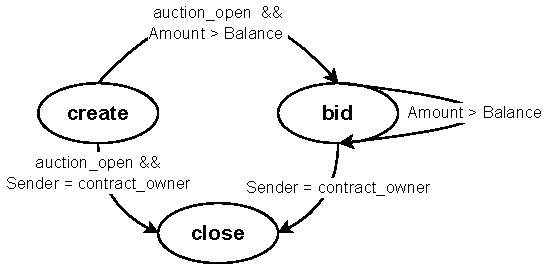
\includegraphics[width=0.8\textwidth]{auction-life-cycle}
    \caption{Auction contract life cycle}
    \label{fig:auction-life-cycle}
\end{figure}

\section {Static Checker}
We verify the contract through symbolic execution against its specifications in the contract module. Symbolic execution involves calculating a symbolic stack at each transition from one Michelson instruction to the next. The symbolic interpreter is fully typed and rejects ill-typed Michelson programs, provided the ill-typed part is reachable from the default entry point. The initial stack is derived from the input pattern for each the entry point. To maintain symbolic values as concrete as possible, some instructions may be deemed unreachable or only reachable under specific conditions. This process yields, for each entry point, a set of final symbolic stacks accompanied by a path condition indicating when this final state is reachable. A state is discarded from the final state space if the path condition is not satisfied, indicating that the path is unreachable. Additionally, for each \FAILWITH\ instruction, we obtain a symbolic value for the reported message and a path condition indicating the reachability of this instruction. We employ the SMT solver Z3  to assess the feasibility of a path condition and to check smart contract properies specifying by pre and post conditions. 

The architecture of the static checker is illustrated in Figure \ref{}. The system comprises three phases. The first phase involves user specification, where users provide the Michelson code of the contract and define the properties that the smart contract should satisfy. Subsequently, the code, along with the input pattern, is input to the interpreter to achieve symbolic execution. The path conditions are then fed into a Z3 converter, which transforms these symbolic terms into Z3 formulas. Concurrently, the property specification, specifically pre and post conditions, also undergoes conversion to Z3 formulas in the intermediate phase. The results of the symbolic execution and Z3 formulas are then input into the static checker, which verifies whether these properties hold for the smart contract implementation. This constitutes the verification phase.

\subsection{User specification}
In the user specification phase, users compose the specification in our domain-specific language using the syntax outlined in Section \ref{sec:domain-specific-language}. Note that Michelson code, whether authored by users, obtained from the Tezos blockchain, or compiled from higher-level languages, can be seamlessly employed within our framework. The specification is subsequently parsed into an Abstract Syntax Tree (AST) in OCaml. The code and the input pattern are then utilized as inputs for the interpreter during the intermediate phase to facilitate symbolic execution. In the next phase, the pre and post predicates are transformed into Z3 formulas by the Z3 converter tool.
\subsection{Michelson interpreter and Z3 converter}
The interpreter implements the execution model described in \ref{sec:symbolic-execution-model}. When provided with a concrete input, the interpreter produces a concrete value. In the presence of symbolic input, the result comprises a set of symbolic states represented as terms in OCaml. Due to Michelson being built in OCaml, the conversion of Michelson types or terms to their OCaml counterparts is straightforward. Each state contains the output stack, which has only one element consisting of an operation list and storage, along with the path conditions represented as predicates in conjunctive form. This output is then fed into the Z3 converter, which handles two different types of terms: assertion terms from the AST representing the pre and post-condition specifications, and terms resulting from the interpreter. We utilize the Z3 library in OCaml to construct this converter. Some adjustments are necessary to convert these terms into Z3 formulas. For example, as there is no natural number type (\TNAT) in Z3, the term is converted as an integer type, accompanied by constraints asserting that it is greater than or equal to zero. Several constants, such as \CAMOUNT, \CBALANCE, \CSENDER\ and cryptographic functions, such as \FSHA, \FHASHKEY\ are predefined in the environment that works for any smart contract specifications.

\paragraph{Dealing with loop formalization}
As mentioned earlier, our execution model formalizes loops symbolically using the \FOLD\ and \FMAP\ functions. This approach has the advantage of allowing us to convert these loops into formulas compatible with certain SMT solvers, such as Z3, which support these functions. Specifically, Z3 provides \lstinline/seq.map fn s/, a map function on sequence \lstinline/s/, and \lstinline/(seq.foldl fn b s)/, a fold function with an initial value \lstinline/b/ on sequence \lstinline/s/. These functions are supported for checking assertions that contain them. Therefore, we can directly convert the symbolic results of loops into formulas in Z3.
\subsection{Static checker}
The static checker now performs the verification process by employing symbolic execution against the property specification in the DSL. It utilizes the results from the previous phases, including symbolic execution, Z3 formulas representing pre and post conditions, and path conditions. 

What the tool does is first build the input state from the input pattern, runs the symbolic interpreter on the input stack with the provided code to generate all symbolic execution states. It's important to note that all states are reachable from the initial state, as any unreachable states are discarded from the final state spaces using the Z3 solver to check the path condition predicate. Using the output pattern and the pre- and post-conditions converted by the Z3 conveter, the tool then performs different checks. The static checker offers three distinct features: output check, fail condition, and property check.

\subsubsection{Output check} 
The first check is the output check, where the checker verifies whether the output pattern matches. The final state contains a stack with only one element as \Stack\ \STACKCONCAT\ \EMPTYSTACK. There are two different forms of the final state. In the case where the code is given as incomplete smart contract code, the element \Stack\ contains just a normal term and its corresponding type as (\Term, \TY). However, in the case of a complete smart contract code, it has the form (\PAIR\ \VOPERATIONLIST\ \VSTORAGE, \TPAIR\ (\TOPERATIONLIST) \TYS) \STACKCONCAT\ \EMPTYSTACK, where \VSTORAGE\ is the term represting the storage and \VOPERATIONLIST\ repesents a operation list. Given an output pattern $ \tau$, the checker scans all the final states, which does not contain a failwith stack and checks whether the output pattern matches. In the former case, it matches $ \tau$  with the term \Term. In the latter case, it essentially matches with the corresponding part \VSTORAGE\ in the final states resulting from the symbolic interpreter. When the input pattern is a concrete value, the result from the interpreter is also concrete, and then the checker can be used as a test to verify if the output aligns with the expectations specified in the output field.

Lets get back to the example in Listing \ref{lst:add-contract-specification}. This is an example of incomplete smart contract code. The specification states that the output of the code must be a stack that contains only one element of type \TINT\ as symbolicly representing as a variable \VZ\ of type \TINT.  In this example, there are two final states, with the first one being a failwith state recording the failwith condition when the first element of the pair is less than the second element. The failwith state contains the message 'Unexpected Pair,' describing the reason for the failure. The second state is a reachable state that contains, at the top element, an integer value, which is the sum of the two elements of the pair. The tool results in \TRUE\ for the output check for this example, as expected by the code. However, this test could fail if, for example, the output pattern is incorrectly specified as a variable of type \TSTRING, \TMUTEZ, or even \TNAT, as the types wouldn't match with the actual result. If the input pattern is concrete, for instance, a pair of numbers 5 and 3 as Pair 5 3, then the expected output should be the number 8. This can be verified if the output pattern is also specified as a concrete value.

The second example in Listing \ref{lst:auction-contract-specification} is the specification for a smart contract code. The output pattern represents the updated storage after executing the code. There are several final states resulting from the symbolic execution. The failwith state is ignored for the output check, and all other reachable states are matched with the output term. The result is \TRUE\ for this example.

\subsubsection{Fail condition}
A Michelson contract can fail due to a programmer-induced condition caused by the instruction \FAILWITH. It terminates contract execution with an error message reported back to the caller. This error message includes the top value on the stack. These failures are important in smart contract programming to guarantee that a smart contract call should not be successful under specific circumstances. Smart contract calls are expected to fail due to malicious behavior, such as an unauthorized caller or invalid arguments passed along the call. For example, the auction contract should not be closed by someone who is not the owner of the contract, and the bidding should not succeed if the bid is not strictly higher than the current highest bid. Several smart contract standards, such as , require the contract to fail with specific messages under some conditions. Therefore, it is essential to check the fail conditions of a contract. 

The static checker provides a feature to generate all fail conditions implemented in a smart contract code. The tool searches for all failwith states, resulting from an execution terminated by the \FAILWITH\ instruction, from the final state space, collects the path conditions and the recorded message. The result returned to users includes the fail condition together with the message. For example, for the specification in Listing \ref{lst:add-contract-specification}, the fail condition is recorded as \lstinline/(x < y): 'Unexpected Pair'/. 

For the auction contract, there are several fail conditions. For the entrypoint \lstinline/bid/, the fail condition is as shown in Listing \ref{lst:fail-condition-auction-contract-bid} and for the \lstinline/close/ entrypoint, it is recorded in Listing \ref{lst:fail-condition-auction-contract-close}. For the \lstinline/bid/ entrypoint, there are three fail conditions. First is if the auction is closed, and then if it is not, the contract checks if the amount is greater than the balance. If not, the call fails as well. The last fail happens when the auction is open, the amount is greater than the balance, but the highest bidder's address is invalid. Note that there are several addresses that are valid as Michelson addresses but are not associated with any real account on the Tezos blockchain, or the parameter's type is not correct, while the transfer can only succeed if it is the given parameter and the address is associated with an account with the correct parameter on the Tezos blockchain. Bidding returns the previous highest bid as part of the transaction where the highest bidder is stored as a value of type address. However, to receive a token transfer, this address must be cast (by the Michelson implementation of the contract) to an implicit contract of Michelson type (\TCONTRACT\ \TUNIT). This cast is unavoidable, as a value of contract type cannot be stored. However, the cast may fail, and its failure leads to an error condition that is reported with a \FAILWITH\ instruction in this implementation. In our framework, this cast fail case is shown in the fail condition, but in the user preconditions, it assumes that they are successfully casted. The \lstinline/close/ entrypoint has similar fail conditions when the auction is closed or the owner's address is uncastable. But the other fail condition is when the auction is open, but the sender who calls this entrypoint is not the owner of the contract, which was stored in the contract owner part.

\begin{lstlisting}[float,captionpos=b,caption={Fail condition for Auction contract bid entrypoint },label={lst:fail-condition-auction-contract-bid},numbers=left]
1. not (auction_open): 'Already closed'
2. (auction_open = true) &&
(Amount <= Balance): 'Not higher than the current highest bid'
3. (auction_open = true) &&
(Amount <= Balance) &&
get_contract (Unit, highest_bidder) = None: 'Invalid address' 
\end{lstlisting}

\begin{lstlisting}[float,captionpos=b,caption={Fail condition for Auction contract close entrypoint},label={lst:fail-condition-auction-contract-close},numbers=left]
1. Not (auction_open): 'Already closed'
2. (auction_open = true) &&
Sender != contract_owner): 'Not owner'
3.  (auction_open = true) &&
(Sender = contract_owner) &&
get_contract (Unit, contract_owner) = None: 'Invalid address'
\end{lstlisting}

In this implementation of the auction contract, the failures are recorded as expected. The contract is designed to fail when the auction is closed, the bid is not greater than the old highest bid, or the caller is not the contract owner when attempting to close the contract as transferring the contract balance to their account as a part of the action.

\subsubsection{Property check}
The static checker enables users to verify smart contract properties by providing pre and post condition specifications. A property is specified with the following clause:  \lstinline/pre-condtion : =/ $\mid$ $\Phi_{i}$ \lstinline/ post-condtion : =/   $\mid$ $\Psi_{j}$. This specification asserts that if all preconditions $\Phi_{i}$ hold before smart contract execution, then all $\Psi_{j}$ must become true after the execution. To verify this property, we explore all the paths $\Pi$ with the path condition $\Theta$ such that ($\bigwedge \Phi_{i}$ $\land$ $\Theta$) is satisfiable. We then check that for every path $\Pi$, $\neg$ ($\bigwedge \Phi_{i} \rightarrow \bigwedge \Psi_{j}$) is unsatisfiable in the context given by the input for the entry point and its corresponding final state and path condition.

Consider the specification of the Add contract in Listing \ref{lst:add-contract-specification}. In this context, the two variables \lstinline/x/ and \lstinline/y/ are integers. The results of the symbolic execution are either a failwith state with the path condition as the predicate stating that the variable \lstinline/x/ is less than \lstinline/y/, or a state in which the final stack has only one element, which is a symbolic variable \lstinline/sbvar/ of type integer, with the path condition stating that the variable \lstinline/x/ is greater than or equal to \lstinline/y/ and the symbolic variable \lstinline/sbvar/ is equal to the sum of \lstinline/x/ and \lstinline/y/. For this specification, the failwith branch is discarded because the precondition is not satisfy with tha path condition, and then \lstinline/z/ is matched to the symbolic variable \lstinline/sbvar/ in the other branch. In this example, the checker then verifies that given the with the context asserting that (\lstinline/x/ >= \lstinline/y/) $\land$ (\lstinline/z/ = \lstinline/x/ + \lstinline/y/), $\neg$ ((\lstinline/x/ >= 5) $\land$ (\lstinline/y/ > 3) $\rightarrow$ (\lstinline/z/ >= 8)) is unsatisfiable. 

\subsubsection{Life-cycle check}
\section {Case Studies}
\subsection{USDtz}
In a blockchain ecosystem, tokens represent digital assets that can be transferred between accounts. These tokens are securely stored and verified within the blockchain network. There are various types of tokens, including native tokens (cryptocurrencies) like Bitcoin, Ether, Tezos, and others. Additionally, tokens can be created through smart contracts on an existing blockchain. Two common categories are: (1) Fungible Tokens (FT), which are interchangeable and (2) Non-Fungible Tokens (NFTs), which represent unique digital assets, and each unit is distinct. Stablecoins, falling under fungible tokens, are designed to maintain a stable value by tracking the value of a fiat currency like USD or EUR.

While you can create tokens that behave in any way that you want them to behave, implementing tokens that adhere to established standards is advisable for interoperability and compatibility across different platforms. A Token standard defines a set of rules and an interface that smart contracts must follow to ensure consistency and compatibility with decentralized exchanges, wallets, and other tools within the ecosystem. For example, ERC-20 is a stoken tandard used in Ethereum. 

Tezos blockchain has its own set of standards known as Financial Applications (FA). Two notable standards are: (1) FA 1.2, designed for fungible tokens, and (2) FA 2, a more versatile standard accommodating both fungible and non-fungible tokens (NFTs).  The standard outlines a smart contract that functions as a ledger, associating identities with balances. This ledger is designed to facilitate token transfer operations and enable approvals for spending tokens from other accounts. Any contract aiming to implement the standard must incorporate the functions specified in Listing \ref{lst:fa12-interface} such as transfer (transacting between users), approve (allowing one user to send tokens from another user's address), allowance (browsing the amount of tokens available for an account to sending from another address), user balance (checking the balance of a user), and current supply (checking the total supply of tokens across all addresses). Further elaboration on the details of FA 1.2 can be found in \ref{}, and we will delve into these functions in subsequent sections.

\begin{lstlisting}[float,captionpos=b,caption={FA 1.2 interface},label={lst:fa12-interface},numbers=left]
(address :from, (address :to, nat :value)) %transfer
(address :spender, nat :value) %approve
(view (address :owner, address :spender) nat) %getAllowance
(view (address :owner) nat) %getBalance
(view unit nat) %getTotalSupply
\end{lstlisting}

In this section, we verify USDtz \ref{}, an implementation of the FA 1.2 standard. Our goal is to ensure that the implementation aligns with the standard, verifying its correctness. USDtz is a stablecoin and one of the first and longest-running coins on the Tezos blockchain, launched in September 2020. The smart contract is located at the address KT1LN4LPSqTMS7Sd2CJw4bbDGRkMv2t68Fy9, and the code can be found on the Tezos blockchain \ref{}. USDtz adheres to the FA token standard, and the initial deployment of the USDtz smart contract follows the FA 1.2 standard.
The implementation consists of approximately 1000 instructions. It contains all of five entrypoints required in the FA 1.2 interface and four others.  We will verify this smart contract for each of its entrypoints.  Let's first examine how the approvable ledger is implemented in the USDtz smart contract. The ledger is a substantial map that links user addresses to a pair consisting of their balance and a map associating addresses with the amount of tokens allowed to be transferred from the user's account. The storage structure of the USDtz smart contract is illustrated in Listing \ref{lst:storage-udstz-contract}. 

\begin{lstlisting}[float,captionpos=b,caption={Storage of the USDtz smart contract},label={lst:storage-udstz-contract},numbers=left]
  ( pair
    ( big_map %ledger
      ( address :user )
      ( pair ( nat :balance ) ( map :approvals
        ( address :spender )
        ( nat :value ) ) ) )
    ( pair ( address %admin ) 
           ( pair ( bool %paused ) ( nat %totalSupply ) ) ) ) 
\end{lstlisting}


\subsubsection{transfer}
As illustrated in Listing \ref{lst:fa12-interface}, the \lstinline/transfer/ entrypoint credits the account associated with the address provided in the \lstinline/to/ parameter, while debiting the account corresponding to the \lstinline/from/ parameter with the specified \lstinline/value/ amount. The FA 1.2 standard mandates that this call must fail under the following two conditions: (1) In the event of insufficient balance, this entrypoint MUST fail with the error \lstinline/NotEnoughBalance/, indicating insufficient funds in the sender's account to execute the transfer. The error MUST contain a \lstinline/pair (nat :value) (nat :present)/ pair, where \lstinline/value/ is the requested amount of tokens, and \lstinline/present/ is the available amount. (2) If the sender's account has no permission to withdraw the \lstinline/value/ amount of funds, the call will fail with the \lstinline/NotEnoughAllowance/ error, which also contains the same pair message as the first failure scenario. To verify these requirements, we utilize the failwith condition feature of the tool and examine the returned results, as outlined in Listing \ref{}.  

The fundamental property that this entrypoint should satisfy is the decrement of the allowance of the sender's account by the \lstinline/value/ that has been sent.

\subsubsection{approve}

\subsubsection{getAllowance, getBalance and  getTotalSupply}
These entrypoints are view entrypoints, and their results, as natural numbers, are sent back to specific addresses, which are smart contracts with entrypoints that have a parameter type of \lstinline/nat/. The property is that there should be no modification in the ledger when these entrypoints are called, and the correct information is sent to the users.

\subsection{Kolibri Oracle Contract}
\section {Conclusion}
\section {Appendix}
\end{document}
